\documentclass[10pt,a4paper]{article}
\usepackage[margin=2cm]{geometry}
\usepackage{amsmath,amssymb}
\usepackage{graphicx,booktabs,xcolor}
\usepackage{listings}
\usepackage[colorlinks=true,linkcolor=blue!50!black,urlcolor=blue!50!black,citecolor=blue!50!black]{hyperref}
\usepackage{microtype}

\lstset{language=Python,basicstyle=\ttfamily\small,keywordstyle=\color{blue!60!black}\bfseries,
  commentstyle=\color{green!40!black},stringstyle=\color{red!50!black},
  frame=single,framerule=0.3pt,rulecolor=\color{gray!60},backgroundcolor=\color{gray!5},
  columns=fullflexible,keepspaces=true,showstringspaces=false,
  numbers=left,numberstyle=\tiny\color{gray},xleftmargin=1.5em,aboveskip=6pt,belowskip=4pt}
\newcommand{\code}[1]{\texttt{#1}}
\newcommand{\Th}{\mathcal{T}_h}
\newcommand{\Fh}{\mathcal{F}_h}
\newcommand{\Div}{\operatorname{div}}
\setlength{\parindent}{0pt}\setlength{\parskip}{4pt}\setlength{\emergencystretch}{3em}\sloppy
\setlength{\textfloatsep}{8pt}\setlength{\intextsep}{7pt}\setlength{\abovecaptionskip}{4pt}\setlength{\belowcaptionskip}{0pt}

\title{\vspace{-1.2cm}The TDNNS Method for Elasticity in NGSolve\\[2pt]
\large Spaces, pairings and the space-creation syntax}
\author{Astrid Pechstein, Michael Neunteufel, Joachim Sch\"oberl}
\date{NGSolve Technical Note 2026-02\quad\textbullet\quad November 2026}

\begin{document}
\maketitle\vspace{-1.2cm}

\section{The method}

We consider linear elasticity on $\Omega\subset\mathbb R^d$, $d=2,3$: find the displacement $u$ and the symmetric stress $\sigma$ with
\[
  A\sigma = \varepsilon(u), \qquad -\Div\sigma = f \quad\text{in }\Omega, \qquad
  A\sigma := \tfrac{1}{2\mu}\bigl(\sigma - \tfrac{\lambda}{2\mu+d\lambda}\operatorname{tr}(\sigma)\,I\bigr),
\]
$u=g$ on $\Gamma_D$ and $\sigma n = t$ on $\Gamma_N$. Here $\varepsilon(u)$ is the symmetric gradient and $\mu,\lambda$ are the Lam\'e parameters.
The tangential-displacement normal-normal-stress (TDNNS) method \cite{sinwel,ps11} uses
\begin{itemize}\setlength\itemsep{1pt}
\item a \emph{tangentially continuous} displacement, $u_h\in V_h\subset H(\operatorname{curl})$ (N\'ed\'elec elements), and
\item a symmetric stress with \emph{continuous normal-normal component} $\sigma_{nn}=n^T\sigma n$, $\sigma_h\in\Sigma_h\subset H(\Div\Div)$.
\end{itemize}
With $w_t := w-(w\cdot n)n$, $w_n:=w\cdot n$ and $\tau_{nt}:=(\tau n)_t$, the method reads: find $(\sigma_h,u_h)\in\Sigma_h\times V_h$ such that
\begin{align*}
  (A\sigma_h,\tau) + \langle\Div\tau,u_h\rangle &= \textstyle\int_{\Gamma_D} g_n\,\tau_{nn}\,ds && \forall\,\tau\in\Sigma_h,\\
  \langle\Div\sigma_h,v\rangle &= -(f,v) - \textstyle\int_{\Gamma_N} t_t\cdot v_t\,ds && \forall\,v\in V_h,
\end{align*}
with the distributional divergence pairing, written element by element in two equivalent ways:
\[
  \langle\Div\tau,v\rangle \;=\; \sum_{T\in\Th}\Bigl(\int_T \Div\tau\cdot v\,dx - \int_{\partial T}\tau_{nt}\cdot v_t\,ds\Bigr)
  \;=\; -\sum_{T\in\Th}\Bigl(\int_T \tau:\varepsilon(v)\,dx - \int_{\partial T}\tau_{nn}\,v_n\,ds\Bigr).
\]
The conditions $u_t=g_t$ and $\sigma_{nn}=t_n$ are essential; $u_n = g_n$ and $\sigma_{nt}=t_t$ are natural.
The method is stable in $h$-dependent and in natural norms \cite{ps11,ps18} and it is suited for anisotropic elements in thin structures \cite{ps12}.

\paragraph{Hybridization.}
The $nn$-continuity of the stress is broken, $\Sigma_h^{dc}=\prod_T\Sigma_h|_T$, and enforced by a multiplier $\hat u_h\in\hat V_h$ on the facets $\Fh$, which is the \emph{normal displacement}. The pairing becomes
\[
  \langle\Div\tau,(v,\hat v)\rangle \;=\; \sum_{T\in\Th}\Bigl(\int_T \Div\tau\cdot v\,dx - \int_{\partial T}\tau_{nt}\cdot v_t\,ds - \int_{\partial T}\tau_{nn}\,\hat v_n\,ds\Bigr).
\]
Now both displacement conditions are essential ($u_t=g_t$ in $V_h$, $\hat u_n=g_n$ in $\hat V_h$) and the whole traction is natural: the right-hand side gets $-\int_{\Gamma_N}(t_t\cdot v_t+t_n\hat v_n)\,ds$. Prescribing only $\hat u_n=0$ gives a sliding condition.
All stress dofs are element-local; static condensation leaves a symmetric positive definite system for $(u_h,\hat u_h)$, after multiplying the equations by $-1$ as in the listing below.

\section{The spaces}

Let $m\ge1$ be the displacement order. The order conventions of \code{HCurl} are those of Technical Note 2026-01 (\emph{High-order de Rham sequences on mixed meshes}): \code{HCurl(m)} has tangential traces of degree $m$ and contains the gradients of \code{H1(m+1)}; \code{type1=True} uses the gradients of \code{H1(m)} only.

\begin{description}\setlength\itemsep{2pt}
\item[Displacement] \code{Q = HCurl(mesh, order=m)} (default, N\'ed\'elec type II on simplices) or \code{HCurl(mesh, order=m, type1=True)}.
\item[Stress] \code{S = Q.CreateStressSpace()} returns an \code{HDivDiv} space of symmetric matrices with continuous $\sigma_{nn}$, mapped by the double Piola transformation. The polynomial degree of $\sigma_{nn}$ on facets and the degree in the element interior are chosen per element type (Table~\ref{tab:rules}). \code{print(S.flags)} shows the choice. Keyword arguments are passed to \code{HDivDiv}; \code{dirichlet="..."} marks the boundary where $\sigma_{nn}$ is essential (conforming method), and an explicit \code{order=...} switches the automatic choice off.
\item[Hybridization] \code{Sdc = Discontinuous(S)} breaks the $nn$-continuity. \code{M = Sdc.CreateMultiplierSpace()} is \code{NormalFacetFESpace} with the facet order of \code{S}: $\hat V_h=\{\hat v\,n:\ \hat v|_F\in P_k(F)\}$ ($Q_k$ on quadrilateral faces). Since the degrees match, the hybrid and the conforming method give the same solution; measured differences are $10^{-13}$ on tets, prisms, tet--prism, prism--hex and trig--quad meshes.
\end{description}

\begin{table}[h]\centering\small
\begin{tabular}{@{}lllcc@{}}\toprule
 element & \code{type1=True} & default \code{HCurl(m)}\quad (single type / in mixed meshes) & $\sigma$ dofs & $u$ dofs\\\midrule
 trig  & $(m{-}1,\,m{-}1)$, \code{plus} & $(m,\,m)$ \ /\ $(m{-}1,\,m)$ & 18 & 12\\
 quad  & $(m{-}1,\,m{-}1)$ & $(m{-}1,\,m{-}1)$, \code{quadfullpol} & 25 & 19\\
 tet   & $(m{-}1,\,m{-}1)$ & $(m{-}1,\,m{-}1)$, \code{plus} & 36 & 30\\
 prism & $(m{-}1,\,m{-}1)$ & $(m,\,m)$ \ /\ $(m{-}1,\,m)$ & 131 & 58\\
 hex   & $(m{-}1,\,m{-}1)$ & $(m{-}1,\,m)$ & 228 & 91\\\bottomrule
\end{tabular}
\caption{Result of \code{CreateStressSpace()} as (facet order, interior order) of \code{HDivDiv}, and element dofs of the default pairing for $m=2$. \code{plus} and \code{quadfullpol} add interior functions. Mixed meshes use the common facet order $m-1$. Orders are at least 1, except for \code{type1}, $m=1$ on meshes without simplices (order 0). Pyramids raise an exception.}\label{tab:rules}
\end{table}

\section{A complete example}

Hybrid TDNNS on unstructured tets, $m=2$, manufactured solution: displacement data on five faces of the unit cube, traction data on the sixth. \code{Solve} detects the local dofs and applies static condensation.

\begin{lstlisting}
from ngsolve import *
from netgen.occ import Box, X
box = Box((0,0,0), (1,1,1))
box.faces.name = "fix"
box.faces.Max(X).name = "load"
mesh = box.GenerateMesh(maxh=0.2)

k, E, nu = 2, 1, 0.3
mu, lam = E/(2*(1+nu)), E*nu/((1+nu)*(1-2*nu))
A = lambda s: 1/(2*mu)*(s - lam/(2*mu+3*lam)*Trace(s)*Id(3))    # compliance

uex = CF((sin(x+y)*(1+z), cos(x)*y+z*z, exp(x)*sin(z)+y))       # manufactured solution
gradu = CF((uex.Diff(x), uex.Diff(y), uex.Diff(z)), dims=(3,3)).trans
sex = 2*mu*Sym(gradu) + lam*Trace(gradu)*Id(3)
f = -CF(tuple(sex[i,0].Diff(x) + sex[i,1].Diff(y) + sex[i,2].Diff(z) for i in range(3)))

Q = HCurl(mesh, order=k)                    # displacement, tangentially continuous
S = Discontinuous(Q.CreateStressSpace())    # stress, nn-continuity broken
M = S.CreateMultiplierSpace()               # normal displacement on facets
(sigma, u, un), (tau, v, vn) = (S*Q*M).TnT()
n = specialcf.normal(3)
tang = lambda w: w - (w*n)*n
nn = lambda s: (s*n)*n
def b(tau, v, vn):                          # -<div tau, (v, vn)>
    return -div(tau)*v*dx + ((tau*n)*tang(v) + nn(tau)*(vn*n))*dx(element_boundary=True)
a = -InnerProduct(A(sigma), tau)*dx + b(tau, u, un) + b(sigma, v, vn)
rhs = f*v*dx + (sex*n)*(tang(v.Trace()) + vn.Trace())*ds("load")
gf = Solve(a == rhs, u[BND("fix")] == uex, un[BND("fix")] == uex)
sigmah, uh, unh = gf.components
err = lambda w: sqrt(Integrate(InnerProduct(w, w), mesh))
print(mesh.ne, gf.space.ndof, gf.space.FreeDofs(True).NumSet(), err(sigmah-sex), err(uh-uex))
\end{lstlisting}

The script prints 648 tets, 35\,289 dofs, of which 11\,961 remain after condensation, and the $L^2$ errors $6.95\cdot10^{-3}$ for $\sigma$ and $2.57\cdot10^{-4}$ for $u$. With \code{maxh} $=0.4,\,0.2,\,0.1$ the errors are $3.72\cdot10^{-2},\ 6.95\cdot10^{-3},\ 1.77\cdot10^{-3}$ for $\sigma$ and $3.04\cdot10^{-3},\ 2.57\cdot10^{-4},\ 3.32\cdot10^{-5}$ for $u$; the finest run (4785 tets, 253\,953 dofs) takes about 3\,s on a laptop.
The boundary term needs the \code{Trace()} of the test functions. The script does not depend on the element type: for structured hexes or prisms, or a mesh with a prism boundary layer, only the mesh lines and boundary names change ($2^3,4^3,8^3$ hexes: $\sigma$-errors $2.04\cdot10^{-2},\ 5.05\cdot10^{-3},\ 1.29\cdot10^{-3}$).

\section{Convergence and choice of the pairing}

Unit square and cube, smooth solution, $\nu=0.3$, hybrid method with Dirichlet data, structured meshes; \emph{trig+quad}: every third cell split, \emph{prism+hex}: alternating columns, \emph{tet+prism}: unstructured tets with a prism boundary layer.

\begin{figure}[h]\centering
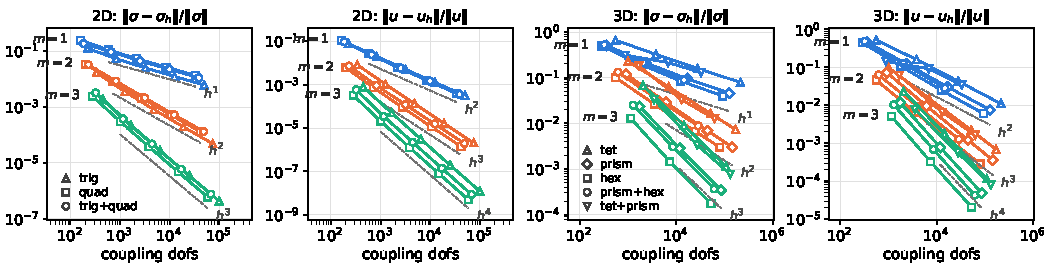
\includegraphics[width=\textwidth]{conv.pdf}\vspace{-2mm}
\caption{Default \code{HCurl(m)} with \code{CreateStressSpace()}: relative $L^2$ errors over the number of coupling dofs. Dashed: optimal rates $h^m$ for $\sigma$ and $h^{m+1}$ for $u$.}\label{fig:conv}
\end{figure}

\begin{table}[h]\centering\footnotesize\setlength{\tabcolsep}{5pt}
\begin{tabular}{@{}l ccc c ccc@{}}\toprule
 & \multicolumn{3}{c}{default \code{HCurl(m)}} && \multicolumn{3}{c}{\code{type1=True}}\\
 mesh & $m=1$ & $m=2$ & $m=3$ && $m=1$ & $m=2$ & $m=3$\\\midrule
 trig      & 1.01 / 2.00 & 2.03 / 3.00 & 3.01 / 4.00 && 0.00 / 0.00 & 1.98 / 2.00 & 3.00 / 3.00\\
 quad      & 1.00 / 2.00 & 2.00 / 3.00 & 3.00 / 4.00 && 1.00 / 1.00 & 1.99 / 2.00 & 3.00 / 3.00\\
 trig+quad & 1.01 / 2.01 & 2.00 / 2.97 & 3.00 / 4.00 && 0.00 / 0.00 & 1.99 / 2.00 & 2.99 / 3.00\\
 tet       & 1.01 / 1.97 & 1.98 / 2.87 & 2.98 / 3.93 && $-$0.01 / 0.00 & 1.07 / 1.98 & 2.04 / 2.97\\
 prism     & 1.05 / 2.00 & 2.05 / 3.00 & 3.04 / 4.01 && 0.69 / 0.34 & 1.34 / 1.08 & 2.65 / 2.38\\
 hex       & 1.08 / 2.04 & 1.98 / 2.90 & 3.04 / 3.98 && 1.00 / 1.01 & 1.95 / 2.01 & 3.00 / 3.01\\
 prism+hex & 1.26 / 2.12 & 1.95 / 2.86 & 3.05 / 4.01 && 0.99 / 1.07 & 1.95 / 2.03 & 2.97 / 3.02\\
 tet+prism & 0.92 / 1.78 & 1.77 / 2.54 & 2.69 / 3.59 && $-$0.12 / $-$0.08 & 0.90 / 1.74 & 1.82 / 2.63\\\bottomrule
\end{tabular}
\caption{Measured rates of $\|\sigma-\sigma_h\|_{L^2}$ / $\|u-u_h\|_{L^2}$ between the two finest meshes ($h=1/64$ in 2D; $h=1/16,\,1/12,\,1/8$ for $m=1,2,3$ in 3D; $1/8$ on the mixed 3D meshes). The tet+prism meshes are unstructured and not nested; their rates are computed from the element counts.}\label{tab:rates}
\end{table}

\begin{itemize}\setlength\itemsep{1pt}
\item \textbf{Default \code{HCurl(m)}} is optimal on every element type and on mixed meshes: $\|\sigma-\sigma_h\|=O(h^m)$, $\|u-u_h\|=O(h^{m+1})$ (Fig.~\ref{fig:conv}, Table~\ref{tab:rates}). This is the recommended pairing.
\item \textbf{\code{type1}} has fewer coupling dofs (in 2D $2m$ per edge instead of $2m+2$ on trigs and $2m+1$ on quads) and gives rate $m$ for $\sigma$ and for $u$ on trigs, quads, hexes and prism--hex meshes. On tets one order is lost in $\sigma$, on prisms the rates degrade under refinement. For $m=1$ on simplices the space consists of element-wise rigid motions and the method does not converge.
\item \textbf{Nearly incompressible materials} (Table~\ref{tab:robust}, left). For $m\ge2$ the relative stress error of the default pairing does not change from $\nu=0.3$ to $\nu=0.499999$ on trigs, quads, tets and hexes, and doubles on prisms. \code{VectorH1} of the same order locks. For $m=1$ the error grows on all types but trigs (quads: $0.18\to0.58$).
\item \textbf{Thin structures} (Table~\ref{tab:robust}, right). With one layer of elements of aspect ratio up to 167, the error for $m\ge2$ does not depend on the thickness $t$. \code{type1} is the most accurate choice on quads, hexes and prisms, but locks on flat tets. $m=1$ has no bending mode and locks (errors $0.2$--$0.8$).
\item \textbf{Non-affine quads and hexes.} Smoothly mapped meshes keep the rates (quads, $m=2$: $2.00/2.99$). If the vertices are moved randomly by $0.2h$ on every level, all pairings lose one order (quads, $m=2$: $1.16/2.06$).
\end{itemize}

\begin{table}[h]\centering\footnotesize\setlength{\tabcolsep}{4pt}
\begin{tabular}{@{}l cc c cc c cc c cc c cc@{}}\toprule
 & \multicolumn{5}{c}{$\|\sigma-\sigma_h\|/\|\sigma\|$ for $\nu=0.3\ \to\ 0.499999$} && \multicolumn{8}{c}{compliance error for $t=10^{-1}\ \to\ 10^{-3}$}\\
 mesh & \multicolumn{2}{c}{TDNNS, $m=2$} && \multicolumn{2}{c}{\code{VectorH1(2)}} && \multicolumn{2}{c}{TDNNS, $m=2$} && \multicolumn{2}{c}{\code{type1}, $m=2$} && \multicolumn{2}{c}{\code{VectorH1(2)}}\\\midrule
 trig  & 6.9e-3 & 7.5e-3 && 2.2e-2 & 1.9 && 2.8e-3 & 5.1e-3 && 3.0e-2 & 1.5e-2 && 2.9e-2 & 3.6e-2\\
 quad  & 8.2e-3 & 8.6e-3 && 9.2e-3 & 3.8 && 9.2e-3 & 5.8e-3 && 3.1e-3 & 1.1e-4 && 1.4e-2 & 2.1e-2\\
 tet   & 8.1e-2 & 8.6e-2 && 1.5e-1 & 3.6 && 7.2e-3 & 1.6e-3 && 8.2e-2 & 5.3e-1 && 4.0e-2 & 6.4e-2\\
 prism & 6.7e-2 & 1.4e-1 && 1.0e-1 & 6.6 && 1.5e-2 & 1.3e-2 && 3.1e-3 & 4.1e-3 && 2.1e-2 & 4.7e-2\\
 hex   & 5.4e-2 & 5.8e-2 && 6.3e-2 & 4.2 && 1.6e-2 & 1.7e-2 && 2.0e-3 & 3.5e-3 && 2.0e-2 & 3.4e-2\\\bottomrule
\end{tabular}
\caption{Left: divergence-free smooth solution, unit square ($16^2$ cells) and cube ($6^3$ cells). Right: cantilever $[0,1]\times[0,t]$ with $8\times1$ cells and plate $[0,1]^2\times[0,t]$ with $6\times6\times1$ cells, clamped at $x=0$, volume load; relative error of the compliance $\int f\cdot u_h$ against a high-order reference (accurate to about $5\cdot10^{-4}$).}\label{tab:robust}
\end{table}

\section{Further developments}

\paragraph{Preconditioning and stabilization.}
The condensed system is solved iteratively by passing \code{preconditioners.BDDC()} and \code{solvers.CGSolver.Creator(tol=1e-8)} to \code{Solve}. Two points matter on tets (Table~\ref{tab:bddc}).
(i) All normal-displacement dofs should be primal: \code{X.SetCouplingType(X.Range(2), COUPLING\_TYPE.WIREBASKET\_DOF)} for \code{X = S*Q*M}. By default one dof per edge and one per face is primal.
(ii) For $\nu\to\frac12$ the element problems lock, although the discrete solution does not. A consistent cure is to add the cubic cell bubbles, \code{Q = HCurl(mesh, order=2, orderinner=3)}, and the constitutive residual
\begin{lstlisting}[numbers=none,xleftmargin=0pt]
eps = lambda w: Sym(Grad(w))
a += 0.1 * 2*mu * InnerProduct(A(sigma)-eps(u), A(tau)-eps(v)) * dx
\end{lstlisting}
The condition number is then independent of $\nu$ and grows slowly under refinement; the $\sigma$-error decreases by 6\,\%.
This stabilization is user code, not a flag of the spaces, and it has been tested for $m=2$ on tets only.

\begin{table}[h]\centering\footnotesize\setlength{\tabcolsep}{5pt}
\begin{tabular}{@{}l ccc c ccc@{}}\toprule
 & \multicolumn{3}{c}{$\nu=0.3$} && \multicolumn{3}{c}{$\nu=0.4999$}\\
 tets & 206 & 648 & 4785 && 206 & 648 & 4785\\\midrule
 default wirebasket                    & 155 (355) & 226 (699) & 363 (4110) && $>$2000 & $>$3000 & $>$3000\\
 (i) normal dofs primal                & 105 (144) & 141 (274) & 183 (463) && $>$2000 & $>$3000 & $>$3000\\
 (i) + (ii) bubbles and residual term  & 64 (49) & 75 (64) & 84 (81) && 68 (55) & 79 (73) & 88 (87)\\\bottomrule
\end{tabular}
\caption{BDDC-preconditioned CG, $m=2$, unstructured tets of the unit cube, Dirichlet data: iterations for a residual reduction of $10^{-8}$ (condition number estimate). With (i), 47\,\% of the coupling dofs are primal.}\label{tab:bddc}
\end{table}

\paragraph{Shells and plates.}
\code{Q.CreateStressSpace(definedon=mesh.Boundaries(...))}, or \code{HCurl} on a surface mesh, returns an \code{HDivDivSurface} space with the trig/quad rules of Table~\ref{tab:rules}. The hybrid version is \code{Discontinuous(S, BND=True)} with \code{CreateMultiplierSpace()} as before; essential conditions use \code{dirichlet\_bbnd}, and \code{sigma.Operator("nncomponent")} is the scalar co-normal component. A plane membrane in 3D reproduces the 2D errors to the four printed digits. The TDNNS Reissner--Mindlin shell (moments in this space, shear in \code{HCurl}) gives the deflection $-0.14998$ for the hyperboloid benchmark with $t=10^{-3}$, order 2, $5\times5\cdot2$ trigs (reference $-0.14989$).

\paragraph{Nonlinear elasticity.}
The three-field methods of \cite{nps21} (unknowns $u$, a stress in \code{HDivDiv}, and the deformation gradient $F$ or the Cauchy--Green tensor $C$ in a discontinuous \code{HCurlCurl} space) can be written with these spaces and symbolic energies; this is research code, not part of NGSolve. For Cook's membrane (neo-Hooke, $\mu=80.194$, $\lambda=40889.8$, load 16, order 2, $16\times16\cdot2$ trigs) the $F$- and the $FC$-based method give the tip deflection $14.154$ (\code{VectorH1(2)}: $14.091$); $FC$ needs 4 Newton steps per load step, $F$ 4--7. They need the full-order stress space of \cite{nps21}: with the reduced quad space of Table~\ref{tab:rules} the $F$-based method fails on $16\times16$ quads.

\section{Open points}
\begin{itemize}\setlength\itemsep{1pt}
\item No \code{HDivDiv} pyramid; no quad or hex stress space without order loss on general non-affine elements.
\item \code{type1}, $m=1$ with stress order 0: the system is singular on prisms with traction boundaries and on one-layer quad or hex meshes with free faces. Use $m\ge2$.
\item Stabilization and wirebasket choice for $m\ge3$ and for prisms and hexes are not settled.
\item \code{plus} has no effect on quads, prisms and hexes; \code{quadfullpol} is an undocumented flag of \code{HDivDiv} (warning if passed explicitly).
\end{itemize}

{\footnotesize\setlength{\itemsep}{0pt}
\begin{thebibliography}{9}\setlength{\itemsep}{1pt}
\bibitem{sinwel} A.~Sinwel. \emph{A New Family of Mixed Finite Elements for Elasticity}. PhD thesis, Johannes Kepler University Linz, 2009.
\bibitem{ps11} A.~Pechstein and J.~Sch\"oberl. Tangential-displacement and normal-normal-stress continuous mixed finite elements for elasticity. \emph{Math. Models Methods Appl. Sci.} 21(8):1761--1782, 2011.
\bibitem{ps12} A.~Pechstein and J.~Sch\"oberl. Anisotropic mixed finite elements for elasticity. \emph{Internat. J. Numer. Methods Engrg.} 90(2):196--217, 2012.
\bibitem{ps18} A.~Pechstein and J.~Sch\"oberl. An analysis of the TDNNS method using natural norms. \emph{Numer. Math.} 139(1):93--120, 2018.
\bibitem{nps21} M.~Neunteufel, A.~Pechstein and J.~Sch\"oberl. Three-field mixed finite element methods for nonlinear elasticity. \emph{Comput. Methods Appl. Mech. Engrg.} 382:113857, 2021.
\end{thebibliography}}

\end{document}
